\documentclass[9pt]{beamer}
\usetheme{Copenhagen}
\usepackage[utf8]{inputenc}
\usepackage[english]{babel}
\usepackage[T1]{fontenc}
\usepackage{amsmath}
\usepackage{amsfonts}
\usepackage{amssymb}
\usepackage{graphicx}
\usepackage{xcolor}
\usepackage{lmodern}
\author{Hjördis Bouvain, Edith Hausten}
\title{The Runge-Kutta-Method for a pendulum}
\setbeamercovered{transparent} 
\setbeamertemplate{navigation symbols}{} 
%\logo{} 
%\institute{} 
%\date{} 
%\subject{} 
\begin{document}

\begin{frame}
\titlepage
\end{frame}

\begin{frame}
\tableofcontents
\end{frame}

\begin{frame}{Pendulum}
\section{Pendulum}
\begin{figure}
\centering
	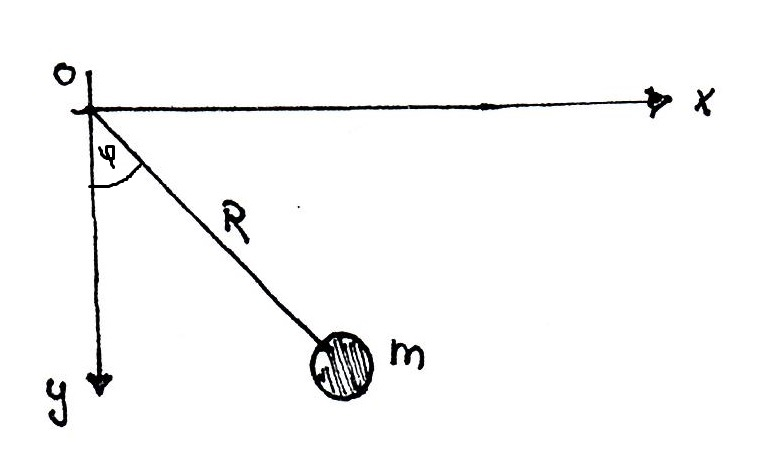
\includegraphics[width=0.5\textwidth]{Pendel.jpg}
	\caption{Pendulum}
\end{figure}
\\
\begin{align*}
&\vec{r} = {x \choose y} = {R\sin\phi \choose R\cos\phi} \qquad L = T-V = \frac{1}{2}mR^2\dot{\phi}^2+mgR\cos\phi 
\\
&\frac{d}{dt}\frac{dL}{d\dot{\phi}}-\frac{dL}{d\phi}=0 \qquad\ddot{\phi}=-\frac{g}{R}\sin{\phi}
\end{align*}
\end{frame}

\begin{frame}{Pendulum - Approximation}
\subsection{Pendulum - Approximation}
\begin{align*}
\sin(\phi) &\approx \phi \\
\ddot{\phi} &= -\frac{g}{R}\phi \\ 
\end{align*}
\\
\begin{center}
\textbf{\fcolorbox{red}{white}{$\phi(t) = \phi_0 \cos(\omega t)$}}
\end{center}
\end{frame}

\begin{frame}{The Runge-Kutta-Method}
\section{The Runge-Kutta-Method}
\begin{itemize}
\item method to solve initial value problems by approximation at discrete positions \\
\item multistep prcedure to reduce the variances
\item most common: 4-step method 
\end{itemize}
\end{frame}

\begin{frame}{The Runge-Kutta-Nyström-Method}
\subsection{The Runge-Kutta-Nyström-Method}
\begin{align*}
k_1 &= \frac{h}{2}f(x_i,y_i,y'_i) \\
k_2 &= \frac{h}{2}f(x_i+\frac{h}{2},y_i\frac{h}{2}y'_i+\frac{h}{4}k_1,y'_i+k_1) \\
k_3 &= \frac{h}{2}f(x_i+\frac{h}{2},y_i+\frac{h}{2}y'_i+\frac{h}{4}k_2,y'_i+k_2) \\
k_4 &= \frac{h}{2}f(x_i+h,y_i+hy'_i+hk_3,y'_i+2k_3) \\
\\
\\
y_{i+1} &= y_i + hy'_i+\frac{h}{3}(k_1+k_2+k_3)\\
y_{i+1} &= y'_i +\frac{1}{3}(k_1+2k_2+2k_3+k_4)\\
\end{align*}
\end{frame}

\begin{frame}{Our Program}
\section{Our Program}

\end{frame}

\begin{frame}{Results}
\section{Results}
\begin{figure}
\centering
	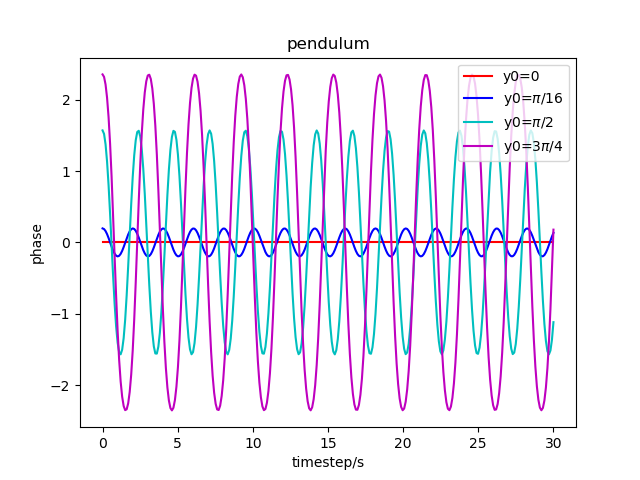
\includegraphics[scale=0.5]{Figure_1.png}
	\caption{Oszillation for various initial angles}
\end{figure}

\end{frame}

\begin{frame}{Results}
\begin{figure}
\centering
	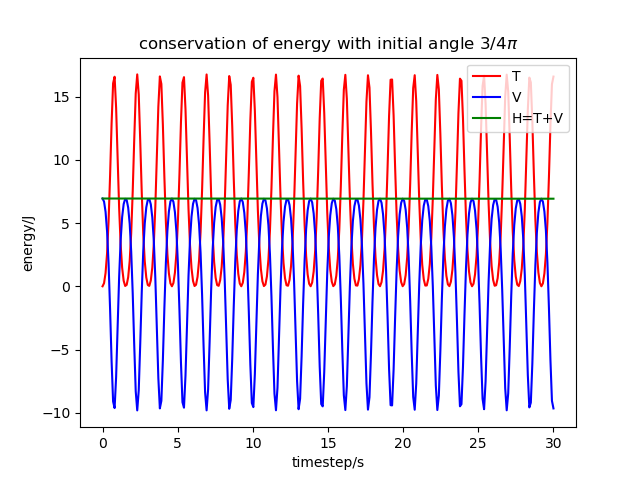
\includegraphics[scale=0.5]{Figure_3.png}
	\caption{Conservation of energy}
\end{figure}

\end{frame}


\begin{frame}
\begin{figure}
\centering
	Thank you for your attention
\end{figure}

\end{frame}

\begin{frame}{Sources}
\section{Sources}
\begin{itemize}
\item http://www.uni-magdeburg.de/ifme/l-numerik/mnmm-2-kapitel%206.pdf
\item https://de.wikipedia.org/wiki/Runge-Kutta-Verfahren
\end{itemize}


\end{frame}



\end{document}